% =============================================================================
% 10-bab1.tex — BAB I PENDAHULUAN
% Patches applied: F1 (remove placeholder), F2 (update goals), C1 (20 tabel)
% =============================================================================
\chapter{PENDAHULUAN}
\label{chap:pendahuluan}

% ─────────────────────────────────────────────────────────────────────────────
\section{Latar Belakang}
\label{sec:latar-belakang}

\textit{Center for Health Psychology} (CHP) adalah unit riset di bawah Program Studi Psikologi, Universitas Kristen Krida Wacana (UKRIDA), yang berperan sebagai pusat rujukan dalam bidang kesehatan mental dan penelitian psikologi klinis. Untuk menjalankan misi tersebut, CHP membutuhkan platform digital yang kokoh, bukan sekadar situs kuis daring, melainkan sebuah instrumen penelitian digital yang harus memenuhi standar validitas dan reliabilitas psikometrik. Prinsip fundamental ini menjadi landasan seluruh keputusan perancangan dalam proyek Kerja Praktik (KP) ini.

% --- Professor-approved: Three manual methods ---
Sebelum proyek ini dimulai, CHP menggunakan tiga metode manual untuk melaksanakan asesmen psikologi. \textbf{Pertama}, metode \textit{paper-based}: responden mengisi lembar jawaban secara manual dan administrator menghitung skor menggunakan panduan penilaian (\textit{scoring guide}) masing-masing instrumen. \textbf{Kedua}, metode \textit{spreadsheet} Excel: administrator mewawancarai responden dan memasukkan data ke dalam lembar kerja Excel; beberapa instrumen telah memiliki rumus otomatis, namun pengelolaan data secara keseluruhan tetap bersifat manual. \textbf{Ketiga}, metode Google Forms: pengumpulan jawaban dilakukan secara daring, namun data harus diekspor terlebih dahulu dan diproses secara manual di luar sistem. Tidak satu pun dari ketiga metode tersebut mampu menyimpan, mengarsipkan, dan memproses data asesmen secara terintegrasi dan otomatis.

% --- Professor-approved: Four operational problems ---
Kondisi ini menimbulkan empat masalah operasional utama:

\begin{enumerate}[leftmargin=2cm]
  \item Proses penilaian yang lambat dan rentan terhadap kesalahan manusia (\textit{human error}), terutama pada instrumen dengan banyak butir soal dan subskala.
  \item Data asesmen tidak tersimpan secara terpusat dan terstruktur, sehingga sulit diakses untuk keperluan penelitian longitudinal.
  \item Tidak tersedia fitur ekspor data berkualitas riset yang kompatibel dengan perangkat lunak analisis statistik seperti SPSS atau JASP.
  \item Asesmen jarak jauh (\textit{remote assessment}) tidak dapat dilaksanakan secara efektif karena ketergantungan pada proses manual.
\end{enumerate}

% --- Professor-approved: Platform capabilities ---
Platform yang dikembangkan dalam proyek KP ini dirancang untuk mengakomodasi seluruh alur kerja asesmen. Responden dapat mengisi asesmen secara daring (\textit{online}) maupun di lokasi (\textit{on-site}). Administrator dapat mengimpor data asesmen manual---baik dari lembar \textit{paper-based} maupun Excel---ke dalam sistem. Seluruh komputasi skor dilakukan secara instan oleh \textit{scoring engine} tanpa intervensi manual. Metode tradisional (\textit{paper-based} atau Excel di lokasi terpencil) tetap dapat digunakan, dan hasilnya dapat diintegrasikan ke dalam platform ketika koneksi tersedia.

Platform ini terdiri atas beberapa modul terintegrasi: modul asesmen yang mengelola siklus hidup pengerjaan tes mulai dari persetujuan peserta hingga komputasi skor; modul administrasi yang menyediakan antarmuka bagi tim psikologi untuk mengelola instrumen, memantau statistik, dan mengekspor data riset; modul autentikasi yang mengimplementasikan sistem keamanan berlapis; serta modul pelaporan yang menghasilkan dokumen hasil asesmen dan mengirimkannya melalui surel.

% --- Professor-approved: Four instrument descriptions ---
Pada tahap awal, platform mengimplementasikan empat instrumen psikometri yang diprioritaskan oleh tim peneliti CHP:

\textbf{\textit{Generalized Problematic Internet Use Scale} 2 (GPIUS-2)} adalah instrumen yang mengukur penggunaan internet bermasalah berdasarkan model kognitif-perilaku. GPIUS-2 terdiri atas 15 butir soal yang terbagi ke dalam lima subskala: \textit{Preference for Online Social Interaction} (POSI), regulasi suasana hati (\textit{mood regulation}), preokupasi kognitif (\textit{cognitive preoccupation}), penggunaan kompulsif (\textit{compulsive use}), dan dampak negatif (\textit{negative outcomes}). Instrumen ini menggunakan skala Likert delapan poin (1--8) dengan rentang skor total 15--120. Rincian butir soal terdapat pada Lampiran~1. Catatan: platform mengimplementasikan versi adaptasi dengan skala Likert 1--5 sesuai keputusan tim peneliti CHP.

\textbf{\textit{Perceived Stress Scale} 10 (PSS-10)} adalah instrumen yang dikembangkan oleh Cohen, Kamarck, dan Mermelstein (1983) untuk mengukur persepsi stres individu \cite{cohen1983}. PSS-10 terdiri atas 10 butir soal yang terbagi ke dalam dua subskala: \textit{perceived helplessness} (6 butir soal) dan \textit{perceived self-efficacy} (4 butir soal terbalik). Instrumen ini menggunakan skala Likert lima poin (0--4) dengan rentang skor total 0--40. PSS-10 telah divalidasi untuk responden berusia 12 tahun ke atas dan telah diterjemahkan ke dalam lebih dari 25 bahasa. Rincian butir soal terdapat pada Lampiran~2.

\textbf{\textit{Self-Reporting Questionnaire} 29 (SRQ-29)} adalah instrumen skrining yang dikembangkan oleh \textit{World Health Organization} (WHO) untuk mendeteksi gangguan kesehatan mental umum. SRQ-29 terdiri atas 29 butir soal dengan format jawaban biner (Ya/Tidak) yang terbagi ke dalam empat domain: somatik, kecemasan, depresi, dan psikosis. Rincian butir soal terdapat pada Lampiran~3.

\textbf{\textit{Stress Response Scale} (SRS)} adalah instrumen yang mengukur kapasitas respons stres individu. SRS terdiri atas 29 butir soal yang terbagi ke dalam tiga dimensi: \textit{self-efficacy}, kepuasan (\textit{satisfaction}), dan kontrol yang dipersepsikan (\textit{perceived control}). Skor yang lebih tinggi mengindikasikan kapasitas regulasi diri yang lebih besar. Rincian butir soal terdapat pada Lampiran~4.

Evaluasi teknis mendalam terhadap sistem web CHP yang sebelumnya dikembangkan oleh tim mahasiswa mengungkapkan sejumlah defisiensi fundamental. Sistem lama dibangun menggunakan \textit{HyperText Markup Language} (HTML), \textit{Cascading Style Sheets} (CSS), dan JavaScript (JS) murni tanpa \textit{framework} apapun, sehingga tidak memiliki struktur arsitektur yang memadai untuk kebutuhan riset jangka panjang. \textit{Technical debt} (akumulasi dampak negatif dari keputusan desain yang tidak optimal) pada sistem lama bersifat struktural, bukan superfisial. Akibatnya, upaya perbaikan tambal sulam akan memakan lebih banyak sumber daya dibandingkan pembangunan ulang dari nol, namun tetap menghasilkan produk yang inferior. Tabel~\ref{tab:defisiensi} merangkum seluruh defisiensi yang ditemukan beserta dampak operasionalnya.

\begin{table}[htbp]
  \centering
  \caption{Defisiensi Sistem CHP Terdahulu}
  \label{tab:defisiensi}
  \begin{tabularx}{\textwidth}{@{}l X X@{}}
    \toprule
    \textbf{Masalah} & \textbf{Deskripsi} & \textbf{Dampak} \\
    \midrule
    Tanpa \textit{Framework} & HTML/CSS/JS murni tanpa struktur arsitektur & Tidak dapat di-\textit{scale}, dipelihara, atau diuji secara sistematis \\
    Struktur File Datar & Semua \textit{file} di direktori root tanpa pemisahan \textit{concerns} & Setiap modifikasi berisiko menyebabkan kegagalan berantai di bagian lain \\
    Tanpa \textit{Type Safety} & JavaScript biasa tanpa \textit{type checking} atau \textit{linting} & \textit{Bug} tersembunyi mencapai produksi tanpa terdeteksi \\
    Cakupan Tes Nol & Tidak ada \textit{unit test}, \textit{integration test}, maupun \textit{end-to-end test} & \textit{Bug} regresi tidak terelakkan pada setiap perubahan kode \\
    Desain Basis Data Tidak Memadai & Skema tidak dapat memodelkan penilaian multidimensional bervariasi & Memblokir fungsionalitas riset inti \\
    Tanpa Dokumentasi & Tidak ada README, dokumentasi API, atau panduan \textit{setup} & Setiap kontributor baru memulai dari nol tanpa acuan \\
    \bottomrule
  \end{tabularx}
\end{table}

Berdasarkan temuan pada Tabel~\ref{tab:defisiensi}, solusi yang dipilih adalah pembangunan ulang total (\textit{full redevelopment}) menggunakan \textit{tech stack} modern berstandar industri. Platform baru dibangun di atas Next.js 16 sebagai \textit{meta-framework} berbasis React, TypeScript sebagai bahasa pemrograman utama yang memberikan keamanan tipe (\textit{type safety}), PostgreSQL sebagai Sistem Manajemen Basis Data Relasional (\textit{Relational Database Management System}/RDBMS), tRPC untuk lapisan API yang aman secara tipe dari ujung ke ujung (\textit{end-to-end type safety}), serta Drizzle \textit{Object-Relational Mapping} (ORM) sebagai lapisan abstraksi basis data. Seluruh sistem di-\textit{deploy} pada platform \textit{serverless} Vercel dengan basis data terkelola melalui Neon PostgreSQL dan \textit{caching} melalui Upstash Redis.

% --- Professor-approved: Updated user groups (3 groups) ---
Sistem yang dibangun melayani tiga kelompok pengguna utama: (1) masyarakat umum termasuk mahasiswa yang membutuhkan asesmen kesehatan mental mandiri (\textit{self-assessment}); (2) administrator dan tim riset psikologi yang mengelola instrumen, memantau sesi, dan mengekspor data berkualitas riset; serta (3) super administrator yang mengelola seluruh akun admin dalam sistem. Metodologi pengembangan yang digunakan adalah Agile iteratif dengan siklus \textit{sprint} dua mingguan, memungkinkan umpan balik berkelanjutan dari pemangku kepentingan di setiap tahap pengembangan. Gambar~\ref{fig:arsitektur-umum} menampilkan gambaran umum arsitektur sistem platform CHP yang dirancang dalam proyek ini.

\begin{figure}[htbp]
  \centering
  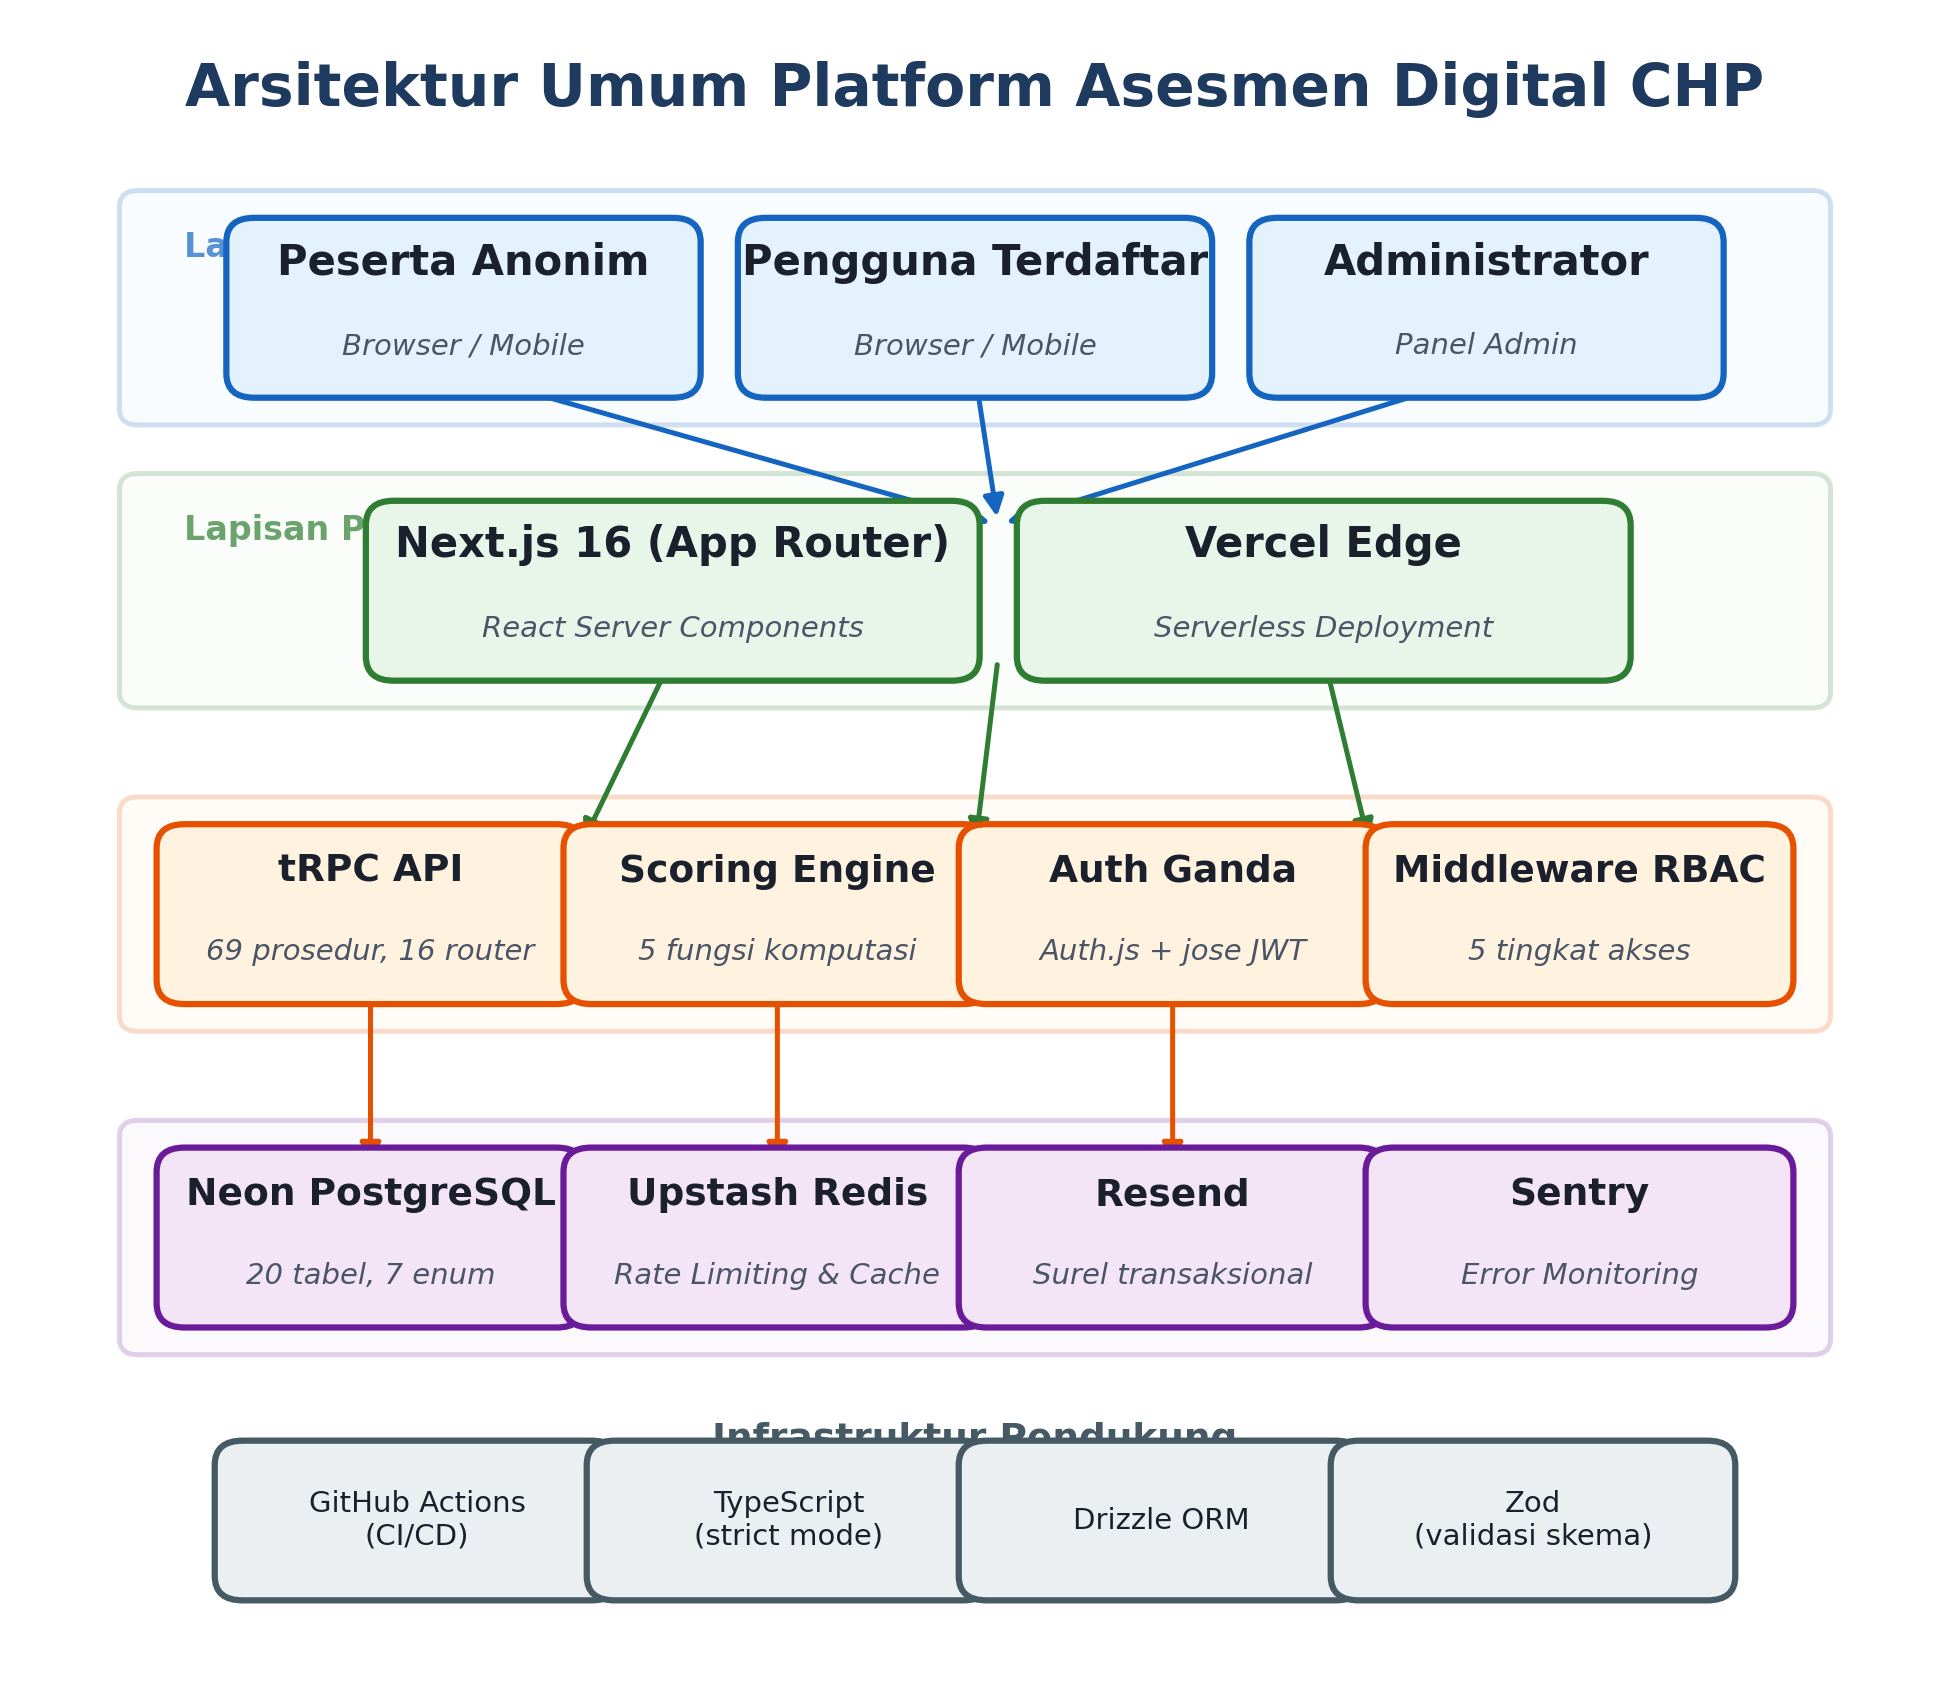
\includegraphics[width=\textwidth]{figures/gambar_1_1_arsitektur_umum.png}
  \caption{Gambaran Umum Arsitektur Platform Asesmen Digital CHP}
  \label{fig:arsitektur-umum}
\end{figure}

% ─────────────────────────────────────────────────────────────────────────────
\section{Skema Kerja Praktik}
\label{sec:skema-kp}

Kerja Praktik (KP) adalah mata kuliah wajib pada Program Studi Informatika UKRIDA yang menekankan aspek kemandirian mahasiswa dalam beradaptasi dengan dunia kerja nyata. Pelaksanaan KP dimaksudkan agar mahasiswa memperoleh pengalaman praktis dalam mengaplikasikan keahliannya di bidang teknologi informasi sekaligus memahami bagaimana suatu instansi dikelola.

KP ini dilaksanakan menggunakan skema Proyek Dosen, yaitu skema di mana mahasiswa terlibat langsung dalam pengembangan produk inovatif milik dosen selaku pemilik proyek. Dosen sebagaimana dimaksud adalah Ibu Astin selaku Ketua Program Studi Psikologi yang sekaligus menjabat sebagai Kepala Riset CHP UKRIDA. Skema Proyek Dosen dipilih karena pengembangan Platform Asesmen Digital CHP merupakan inisiatif riset resmi CHP yang membutuhkan produk \textit{Information Technology} (IT) berupa platform asesmen psikometri digital berkualitas produksi (\textit{production-ready}).

Dalam kerangka proyek ini, penulis bertanggung jawab atas tiga ranah pengembangan utama, yaitu:

\begin{enumerate}[leftmargin=2cm]
  \item Arsitektur sistem: perancangan skema basis data, infrastruktur \textit{Continuous Integration/Continuous Deployment} (CI/CD), dan konfigurasi layanan \textit{cloud}.
  \item \textit{Backend} dan API: implementasi prosedur tRPC, \textit{scoring engine}, dan sistem autentikasi.
  \item Pengujian dan implementasi (\textit{testing and implementation}).
\end{enumerate}

Pengembangan komponen antarmuka pengguna (\textit{User Interface}/UI) dan desain pengalaman pengguna (\textit{User Experience}/UX) dikerjakan secara terpisah oleh anggota tim lain dalam laporan KP tersendiri, sehingga kedua laporan saling melengkapi untuk menggambarkan sistem secara menyeluruh.

% ─────────────────────────────────────────────────────────────────────────────
\section{Tujuan dan Manfaat}
\label{sec:tujuan-manfaat}

Pelaksanaan KP ini memiliki enam tujuan yang dirumuskan menggunakan pendekatan SMART (\textit{Specific, Measurable, Achievable, Relevant, Time-bound}), yaitu spesifik, terukur, dapat dicapai, relevan, dan berbatas waktu. Tabel~\ref{tab:tujuan-kp} menyajikan rumusan tujuan beserta target terukur dan status implementasi pada saat laporan ini disusun.

% [F2] Goals #2, #4, #5, #6 status updated
\begin{longtable}{@{}c p{4cm} p{4.5cm} p{4cm}@{}}
  \caption{Tujuan Kerja Praktik dan Status Implementasi}
  \label{tab:tujuan-kp} \\
  \toprule
  \textbf{No.} & \textbf{Tujuan} & \textbf{Target Terukur} & \textbf{Status} \\
  \midrule
  \endfirsthead
  \toprule
  \textbf{No.} & \textbf{Tujuan} & \textbf{Target Terukur} & \textbf{Status} \\
  \midrule
  \endhead
  \bottomrule
  \endfoot
  1 & Membangun platform asesmen modern dan responsif sesuai standar aksesibilitas & Skor \textit{Lighthouse Performance} $\geq$ 90; \textit{Accessibility} $\geq$ 95 pada semua halaman utama & Selesai: Fase 1A \& 1B (Minggu 1--6) \\[0.5em]
  2 & Mengimplementasikan \textit{scoring engine} modular otomatis untuk perhitungan sumatif, berbobot, dimensional, dan persentil & Skor komputasi sesuai nilai referensi manual; \textit{engine} diuji dengan 72 kasus uji & Selesai: Fase 1B (Minggu 3--6) \\[0.5em]
  3 & Menyajikan umpan balik visual instan berupa skor total, \textit{breakdown} dimensi, dan grafik & Halaman hasil ter-\textit{render} dalam dua detik setelah pengiriman tes & Selesai: Fase 1B (Minggu 5--6) \\[0.5em]
  4 & Membangun fungsionalitas ekspor data berkualitas riset dalam format CSV & Prosedur \texttt{adminResults.export} dengan batas 5000 baris, mencakup jawaban per butir soal & Selesai: Fase 1C (Minggu 7--10) \\[0.5em]
  5 & Mengembangkan panel administrator dengan RBAC & Tim psikologi dapat membuat, mengkonfigurasi, dan mempublikasikan instrumen baru tanpa intervensi pengembang; empat peran admin & Selesai: Fase 1C (Minggu 7--10) \\[0.5em]
  6 & Memastikan serah terima sistem yang berkelanjutan dengan dokumentasi komprehensif & Pengembang baru dapat \textit{clone}, \textit{setup}, dan menjalankan proyek secara lokal dalam waktu 15 menit & Selesai: Fase 1D (Minggu 11--13) \\
\end{longtable}

Adapun manfaat yang diharapkan dari pengembangan Platform Asesmen Digital CHP mencakup empat dimensi utama:

\begin{enumerate}[leftmargin=2cm]
  \item Validitas riset yang meningkat berkat penyimpanan respons mentah yang tidak dapat diubah (\textit{immutable raw responses}) disertai metadata versi instrumen dan versi algoritma penilaian untuk reprodusibilitas ilmiah.
  \item Pengalaman pengguna yang profesional dan aksesibel dengan antarmuka yang menenangkan (\textit{calm design}) sehingga meminimalkan kecemasan peserta tes.
  \item Skalabilitas sistem: untuk menambahkan instrumen psikologi baru secara mandiri melalui panel admin tanpa memerlukan intervensi pengembang.
  \item Keberlanjutan operasional lintas semester: berkat arsitektur yang terdokumentasi secara komprehensif dan kode yang aman secara tipe.
\end{enumerate}

% ─────────────────────────────────────────────────────────────────────────────
\section{Batasan Kerja Praktik}
\label{sec:batasan-kp}

Agar pengerjaan proyek tetap terfokus dan dapat diselesaikan dalam batas waktu yang ditentukan, ruang lingkup pekerjaan ditetapkan sebagai berikut.

Pekerjaan yang termasuk dalam ruang lingkup KP penulis adalah:

\begin{enumerate}[leftmargin=2cm]
  \item Perancangan dan implementasi skema basis data relasional menggunakan Drizzle ORM yang mendukung instrumen psikometri multidimensional, manajemen sesi anonim, dan jejak audit administratif.
  \item Pengembangan infrastruktur CI/CD otomatis menggunakan GitHub Actions dengan dua \textit{job} paralel: \textit{job} pertama menjalankan \textit{linting} (ESLint), \textit{type checking} (TypeScript \textit{Compiler}), dan \textit{build} produksi; \textit{job} kedua menjalankan \textit{unit testing} (Vitest).
  \item Implementasi \textit{scoring engine} modular yang mendukung algoritma penilaian sumatif, berbobot, terbalik (\textit{reversed}), dimensional, dan persentil, sepenuhnya dikonfigurasi melalui basis data.
  \item Pengembangan prosedur API berbasis tRPC untuk manajemen sesi asesmen, penyimpanan jawaban, komputasi skor, autentikasi administrator, dan manajemen instrumen.
  \item Implementasi sistem autentikasi ganda: Auth.js v5 untuk pengguna publik dan JWT mandiri melalui jose untuk panel administrator, dengan \textit{Role-Based Access Control} (RBAC) berlima tingkat.
  \item Pengujian komprehensif mencakup \textit{unit test} pada \textit{scoring engine} dan prosedur API, \textit{integration test} prosedur API, serta pengujian keamanan dasar menggunakan \textit{checklist} OWASP \textit{Top Ten}.
\end{enumerate}

Pekerjaan yang tidak termasuk dalam ruang lingkup KP ini adalah:

\begin{enumerate}[leftmargin=2cm]
  \item Pengembangan aplikasi \textit{mobile native} (iOS/Android): platform bersifat berbasis web (\textit{web-based}) dan responsif untuk perangkat seluler.
  \item Interpretasi hasil berbasis kecerdasan buatan (AI) atau \textit{Large Language Model} (LLM).
  \item Fungsionalitas diagnosis klinis: platform hanya menyediakan \textit{self-assessment} mandiri, bukan diagnosis klinis.
  \item Pengembangan komponen UI dan desain UX, yang merupakan tanggung jawab anggota tim lain dalam laporan KP terpisah.
  \item Fitur aksesibilitas khusus seperti dukungan \textit{screen reader} atau teknologi asistif untuk penyandang disabilitas: fitur ini berada di luar cakupan versi ini dan dicatat sebagai batasan sistem yang dapat dikembangkan pada iterasi berikutnya.
  \item Verifikasi usia responden: sistem tidak membatasi usia pengguna dan tidak dapat memverifikasi apakah responden di bawah umur didampingi oleh orang dewasa. Ini merupakan batasan yang disadari (\textit{known limitation}) dan pengguna diasumsikan mampu membaca instruksi secara mandiri serta mengoperasikan perangkat masukan.
\end{enumerate}

% ─────────────────────────────────────────────────────────────────────────────
\section{Waktu Pelaksanaan}
\label{sec:waktu-pelaksanaan}

Pelaksanaan KP ini berlangsung selama kurang lebih 12 hingga 14 minggu, dimulai pada 11 Februari 2026 melalui koordinasi perdana dengan dosen pemilik proyek hingga direncanakan selesai pada awal Juni 2026 dengan sidang KP. Tabel~\ref{tab:jadwal-kp} menyajikan rincian jadwal pelaksanaan per fase beserta kegiatan utama masing-masing.

% [C1] Changed "16 tabel" → "20 tabel"
\begin{longtable}{@{}p{3.5cm} p{3cm} p{8cm}@{}}
  \caption{Jadwal Pelaksanaan Kerja Praktik}
  \label{tab:jadwal-kp} \\
  \toprule
  \textbf{Fase} & \textbf{Periode} & \textbf{Kegiatan Utama} \\
  \midrule
  \endfirsthead
  \toprule
  \textbf{Fase} & \textbf{Periode} & \textbf{Kegiatan Utama} \\
  \midrule
  \endhead
  \bottomrule
  \endfoot
  Fase 0: Perencanaan & 11 Feb 2026 & Koordinasi perdana, penyusunan rencana proyek (731 baris \textit{unified project plan}), analisis sistem lama \\[0.3em]
  Fase 1A: Fondasi \& \textit{Setup} & Minggu 1--2 & Inisialisasi proyek Next.js, desain skema basis data (20 tabel), konfigurasi CI/CD, \textit{seeding} data awal \\[0.3em]
  Fase 1B: Inti Asesmen & Minggu 3--6 & Katalog tes, mesin asesmen multi-langkah, \textit{scoring engine}, prosedur tRPC, \textit{pre-test} dan \textit{post-test flow} \\[0.3em]
  Fase 2A--2C: Autentikasi & Minggu 4--7 & Infrastruktur JWT ganda, UI autentikasi (\textit{sign-up}, \textit{login}), mutasi \textit{claim session}, migrasi skema Auth.js \\[0.3em]
  Fase 1C: Admin \& \textit{Polish} & Minggu 7--10 & Panel admin dengan RBAC empat peran, CRUD instrumen tes, konfigurasi penilaian, ekspor data \\[0.3em]
  Fase 1D: Pengujian \& Serah Terima & Minggu 11--13 & Pengujian unit (235 kasus uji), pengujian keamanan (OWASP \textit{checklist}), dokumentasi teknis, \textit{deployment} final \\[0.3em]
  Sidang KP & Juni 2026 & Presentasi dan evaluasi akhir di hadapan tim penguji Program Studi Informatika UKRIDA \\
\end{longtable}
